\section{Auswertung}
\label{sec:Auswertung}

\subsection{Braggbedingung}

\begin{figure}[H]
  \centering
  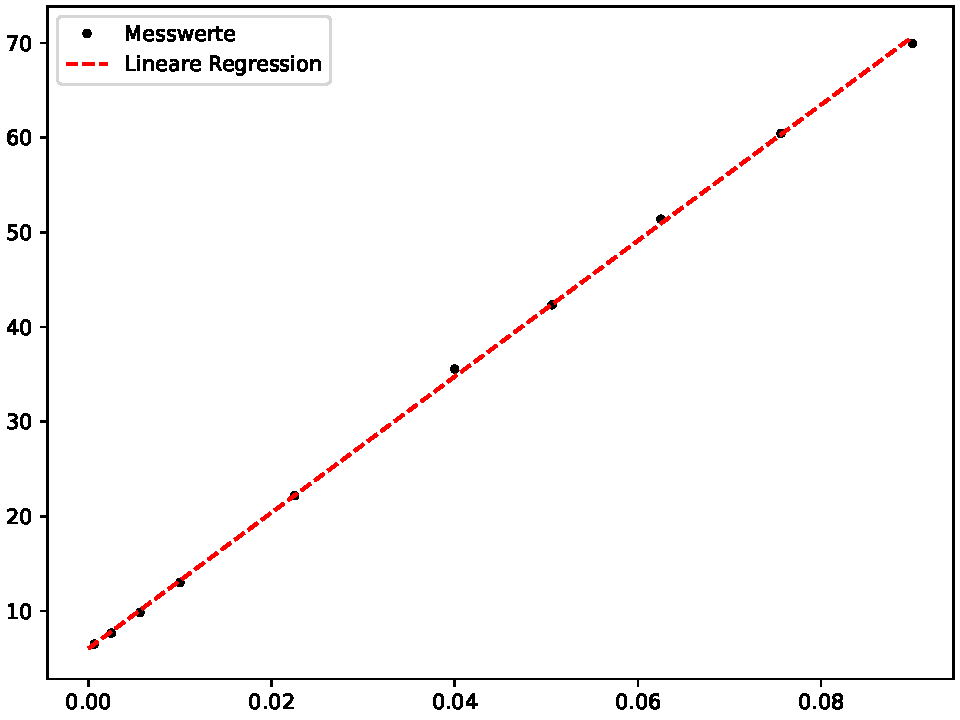
\includegraphics{build/plot.pdf}
  \caption{Messung des Braggwinkels}
  \label{fig:bragg}
\end{figure}

\begin{table}[H]
  \centering
  \caption{Messdaten zum Braggwinkel.}
  \label{tab:bragg}
  \sisetup{table-format=1.1, per-mode=reciprocal}
  \begin{tblr}{
      colspec = {S[table-format=2.1] S[table-format=2.1] },
      row{1} = {guard, mode=math},
    }
    \toprule
    2 \cdot \theta \mathbin{/} ° & R \mathbin{/} \unit{\per\second}\\
    \midrule
    26.0  & 12.0  \\
    26.2  & 16.0  \\
    26.4  & 23.0  \\
    26.6  & 32.0  \\
    26.8  & 46.0  \\
    27.0  & 62.0  \\
    27.2  & 66.0  \\
    27.4  & 74.0  \\
    27.6  & 80.0  \\
    27.8  & 88.0  \\
    28.0  & 85.0  \\
    28.2  & 82.0  \\
    28.4  & 68.0  \\
    28.6  & 60.0  \\
    28.8  & 47.0  \\
    29.0  & 36.0  \\
    29.2  & 32.0  \\
    29.4  & 27.0  \\
    29.6  & 15.0  \\
    29.8  & 13.0  \\
    30.0  & 10.0  \\
    \bottomrule
  \end{tblr}
\end{table}

Der Braggwinkel sollte theoretisch $\theta=14°$ betragen. Aus Abbildung \ref{fig:bragg} und Tabelle \ref{tab:bragg}
lässt sich ein Winkel von $\theta_e=13.8°$ bestimmen. Mit einer Abweichung von $\qty{1.43}{\percent}$ lässt sich dieser
Unterschied vernachlässigen und es kann davon ausgegangen werden, dass die Braggbedingung erfüllt ist.


\subsection{Bestimmung des Kupferemissionsspektrums.}

\begin{figure}[H]
  \centering
  \includegraphics{build/emiss.pdf}
  \caption{Messung des Kupferemissionsspektrum}
  \label{fig:kupfer}
\end{figure}

\begin{table}[H]
	\centering
	\caption{Messdaten zum Kupferemissionsspektrum.}
	\label{tab:kupfer}
	\sisetup{table-format=1.2}
	\begin{tblr}{colspec={S[table-format=2.1] S[table-format=2.0] || S[table-format=2.1] S[table-format=3.0] || S[table-format=2.1] S[table-format=3.0] || S[table-format=2.1] S[table-format=4.0]}, row{1} = {guard, mode=math},
		}
		\toprule
		2 \cdot \theta  \mathbin{/} \unit{ \unit{\degree}} & R  \mathbin{/} \unit{ \unit{\second^{-1}}} & 2 \cdot \theta  \mathbin{/} \unit{ \unit{\degree}} & R  \mathbin{/} \unit{ \unit{\second^{-1}}} & 2 \cdot \theta  \mathbin{/} \unit{ \unit{\degree}} & R  \mathbin{/} \unit{ \unit{\second^{-1}}} & 2 \cdot \theta  \mathbin{/} \unit{ \unit{\degree}} & R  \mathbin{/} \unit{ \unit{\second^{-1}}} \\
		\midrule
		8.0 & 10 & 19.2 & 85 & 30.4 & 78 & 41.5 & 63 \\
		8.3 & 10 & 19.6 & 89 & 30.8 & 70 & 42.0 & 62 \\
		8.8 & 12 & 20.0 & 89 & 31.2 & 75 & 42.4 & 64 \\
		9.2 & 10 & 20.4 & 90 & 31.6 & 76 & 42.8 & 58 \\
		9.6 & 12 & 20.7 & 94 & 32.0 & 76 & 43.2 & 64 \\
		10.0 & 20 & 21.2 & 95 & 32.4 & 70 & 43.5 & 72 \\
		10.4 & 28 & 21.6 & 93 & 32.8 & 70 & 44.0 & 146 \\
		10.8 & 38 & 22.0 & 102 & 33.2 & 63 & 44.4 & 1920 \\
		11.2 & 45 & 22.4 & 96 & 33.5 & 64 & 44.8 & 2270 \\
		11.6 & 53 & 22.7 & 98 & 34.0 & 67 & 45.2 & 1290 \\
		12.0 & 59 & 23.2 & 96 & 34.4 & 63 & 45.5 & 86 \\
		12.4 & 56 & 23.6 & 99 & 34.8 & 65 & 46.0 & 61 \\
		12.8 & 65 & 24.0 & 95 & 35.2 & 58 & 46.4 & 44 \\
		13.2 & 68 & 24.4 & 97 & 35.5 & 52 & 46.8 & 43 \\
		13.6 & 71 & 24.8 & 96 & 36.0 & 52 & 47.2 & 37 \\
		14.0 & 74 & 25.2 & 100 & 36.4 & 54 & 47.5 & 41 \\
		14.4 & 78 & 25.6 & 101 & 36.8 & 58 & 48.0 & 39 \\
		14.8 & 80 & 26.0 & 89 & 37.2 & 57 & 48.4 & 35 \\
		15.2 & 85 & 26.4 & 87 & 37.5 & 50 & 48.8 & 36 \\
		15.6 & 83 & 26.8 & 91 & 38.0 & 52 & 49.2 & 28 \\
		16.0 & 74 & 27.2 & 83 & 38.4 & 52 & 49.6 & 28 \\
		16.4 & 79 & 27.6 & 90 & 38.8 & 46 & 50.0 & 29 \\
		16.7 & 84 & 28.0 & 90 & 39.2 & 53 & 50.4 & 24 \\
		17.2 & 92 & 28.4 & 81 & 39.5 & 112 & 50.8 & 22 \\
		17.6 & 79 & 28.8 & 82 & 40.0 & 607 & 51.2 & 25 \\
		18.0 & 79 & 29.2 & 75 & 40.4 & 641 & 51.6 & 27 \\
		18.4 & 93 & 29.6 & 79 & 40.8 & 101 & 52.0 & 26 \\
		18.7 & 87 & 30.0 & 77 & 41.2 & 83 &   &   \\
		\bottomrule
	\end{tblr}
\end{table}

Hier lassen sich anhand der Tabelle \ref{tab:kupfer} die $\text{K}_{\alpha}$ und $\text{K}_{\beta}$ ablesen.
Also beträgt $\theta_{\alpha}=\qty{22.4(0.2)}°$ und $\theta_{\beta}=\qty{20.2(0.2)}°$. Die Unsicherheit kommt daher,
dass sich das Maximum möglicherweise nicht genau auf dem gemessenen Wert liegt, sondern etwas daneben. Bei der Bestimmung
der Wellenlänge wird dann hier ausschließlich die erste Beugungsebene verwendet. Die $\text{K}_{\alpha}$-Linie
hat somit eine Wellenlänge von $\lambda_{\alpha}=\qty{153.5(1.3)}{\pico\meter}$ mit einer Energie von 
$E_{\alpha}=\qty{8.08(0.07)}{\kilo\electronvolt}$ und die $\text{K}_{\beta}$-Linie eine Wellenlänge von
$\lambda_{\beta}=\qty{139.1(1.3)}{\pico\meter}$ und eine Energie $E_{\beta}=\qty{8.91(0.08)}{\kilo\electronvolt}$.\\
\noindent Um die Genauigkeit des Versuchs abzuschätzen wird die Halbwärtsbreite um die beiden Maxima mithilfe von jeweils
zwei linearen Regressionen berechnet. Bei der $\text{K}_{\beta}$-Linie beträgt dieses $\increment E_{\beta}=\qty{0.286(5)}{\kilo\electronvolt}$
und der  $\text{K}_{\alpha}$-Linie $\increment E_{\alpha}=\qty{0.250(4)}{\kilo\electronvolt}$. Zwar unterscheiden diese
Werte sich, allerdings sind beide groß genug, um behaupten zu können, dass die statsitischen Fehler in den $E_{\symup{i}}$
vernachlässigbar sind. Also gilt $E_{\alpha}=\qty{8.08}{\kilo\electronvolt}$ und $E_{\beta}=\qty{8.91}{\kilo\electronvolt}$.\\
\noindent Daraus lassen sich mithilfe von $E_{abs}=\qty{8.98}{\kilo\electronvolt}$ und den Gleichungen \ref{eqn:Bindungsenergie}
und \ref{eqn:Übergangsenergie} die Absorptionskonstanten $\sigma_{\symup{i}}$ bestimmen. Es sind $\sigma_{abs}=3.30$,
$\sigma_{\alpha}=12.73$ und $\sigma_{\beta}=22.19$.

\subsection{Absorptionsspektren}
\subsection{K-Linie von Brom}

\begin{table}[H]
  \centering
  \caption{Messdaten zum Absorptionsspektrum von Brom.}
  \label{tab:brom}
  \sisetup{table-format=1.1, per-mode=reciprocal}
  \begin{tblr}{
      colspec = {S[table-format=2.1] S[table-format=2.1] },
      row{1} = {guard, mode=math},
    }
    \toprule
    2 \cdot \theta \mathbin{/} ° & R \mathbin{/} \unit{\per\second}\\
    \midrule
    24.4  &	  6.0 \\
    24.8  &	  6.0 \\
    25.2  &	  6.0 \\
    25.6  &	  7.0 \\
    26.0  &	  9.0 \\
    26.4  &	  13.0\\
    26.8  &	  14.0\\
    27.2  &	  13.0\\
    27.6  &	  14.0\\
    28.0  &	  12.0\\
    28.4  &	  10.0\\
    \bottomrule
  \end{tblr}
\end{table}

\begin{figure}[H]
  \centering
  \includegraphics{build/brom.pdf}
  \caption{Messdaten zum Absorptionsspektrum von Brom.}
  \label{fig:brom}
\end{figure}

Mit einem Winkel von etwa 13° ergibt sich hier eine Energie für die $\text{K}_{\alpha}$-Linie von 
$E_{\symup{k}}=\qty{13.68}{\kilo\electronvolt}$.

\subsection{K-Linie von Gallium}

\begin{table}[H]
  \centering
  \caption{Messdaten zum Absorptionsspektrum von Gallium.}
  \label{tab:gallium}
  \sisetup{table-format=1.1, per-mode=reciprocal}
  \begin{tblr}{
      colspec = {S[table-format=2.1] S[table-format=2.1] },
      row{1} = {guard, mode=math},
    }
    \toprule
    2 \cdot \theta \mathbin{/} ° & R \mathbin{/} \unit{\per\second}\\
    \midrule
    32.5  & 	14.0\\
    33.0  & 	13.0\\
    33.4  & 	13.0\\
    33.8  & 	12.0\\
    34.2  & 	17.0\\
    34.5  & 	25.0\\
    35.0  & 	29.0\\
    35.4  & 	27.0\\
    35.8  & 	26.0\\
    36.2  & 	27.0\\
    36.5  & 	25.0\\
    \bottomrule
  \end{tblr}
\end{table}

\begin{figure}[H]
  \centering
  \includegraphics{build/gallium.pdf}
  \caption{Messdaten zum Absorptionsspektrum von Gallium.}
  \label{fig:gallium}
\end{figure}

Mit einem Winkel von etwa 17,25° ergibt sich hier eine Energie für die $\text{K}_{\alpha}$-Linie von 
$E_{\symup{s}}=\qty{10.38}{\kilo\electronvolt}$.

\subsection{K-Linie von Strontium}

\begin{table}[H]
  \centering
  \caption{Messdaten zum Absorptionsspektrum von Strontium.}
  \label{tab:strontium}
  \sisetup{table-format=1.1, per-mode=reciprocal}
  \begin{tblr}{
      colspec = {S[table-format=2.1] S[table-format=2.1] },
      row{1} = {guard, mode=math},
    }
    \toprule
    2 \cdot \theta \mathbin{/} ° & R \mathbin{/} \unit{\per\second}\\
    \midrule
    20.2  & 14.0\\
    20.6  & 14.0\\
    21.0  & 14.0\\
    21.4  & 17.0\\
    21.7  & 23.0\\
    22.2  & 39.0\\
    22.6  & 37.0\\
    23.0  & 38.0\\
    23.4  & 37.0\\
    23.8  & 35.0\\
    24.2  & 34.0\\
    \bottomrule
  \end{tblr}
\end{table}

\begin{figure}[H]
  \centering
  \includegraphics{build/strontium.pdf}
  \caption{Messdaten zum Absorptionsspektrum von Strontium.}
  \label{fig:strontium}
\end{figure}

Mit einem Winkel von etwa 11° ergibt sich hier eine Energie für die $\text{K}_{\alpha}$-Linie von 
$E_{\symup{s}}=\qty{16.13}{\kilo\electronvolt}$.

\subsection{K-Linie von Zink}

\begin{table}[H]
  \centering
  \caption{Messdaten zum Absorptionsspektrum von Zink.}
  \label{tab:zink}
  \sisetup{table-format=1.1, per-mode=reciprocal}
  \begin{tblr}{
      colspec = {S[table-format=2.1] S[table-format=2.1] },
      row{1} = {guard, mode=math},
    }
    \toprule
    2 \cdot \theta \mathbin{/} ° & R \mathbin{/} \unit{\per\second}\\
    \midrule
    35.4&	18.0\\
    35.8&	17.0\\
    36.2&	15.0\\
    36.5&	18.0\\
    37.0&	27.0\\
    37.4&	33.0\\
    37.8&	30.0\\
    38.2&	31.0\\
    38.5&	30.0\\
    39.0&	28.0\\
    39.4&	41.0\\
    \bottomrule
  \end{tblr}
\end{table}

\begin{figure}[H]
  \centering
  \includegraphics{build/zink.pdf}
  \caption{Messdaten zum Absorptionsspektrum von Zink.}
  \label{fig:zink}
\end{figure}

Mit einem Winkel von etwa 18,5° ergibt sich hier eine Energie für die $\text{K}_{\alpha}$-Linie von 
$E_{\symup{z}}=\qty{9.70}{\kilo\electronvolt}$.

\subsection{K-Linie von Zirkonium}

\begin{table}[H]
  \centering
  \caption{Messdaten zum Absorptionsspektrum von Zirkonium.}
  \label{tab:zirkonium}
  \sisetup{table-format=1.1, per-mode=reciprocal}
  \begin{tblr}{
      colspec = {S[table-format=2.1] S[table-format=2.1] },
      row{1} = {guard, mode=math},
    }
    \toprule
    2 \cdot \theta \mathbin{/} ° & R \mathbin{/} \unit{\per\second}\\
    \midrule
    17.7&	35.0\\
    18.2&	34.0\\
    18.6&	32.0\\
    19.0&	35.0\\
    19.4&	49.0\\
    19.7&	59.0\\
    20.2&	60.0\\
    20.6&	64.0\\
    21.0&	64.0\\
    21.4&	62.0\\
    21.7&	65.0\\
    \bottomrule
  \end{tblr}
\end{table}

\begin{figure}[H]
  \centering
  \includegraphics{build/zirkonium.pdf}
  \caption{Messdaten zum Absorptionsspektrum von Zirkonium.}
  \label{fig:zirkonium}
\end{figure}

Mit einem Winkel von etwa 9,75° ergibt sich hier eine Energie für die $\text{K}_{\alpha}$-Linie von 
$E_{\symup{zr}}=\qty{18.18}{\kilo\electronvolt}$.

\subsection{Bestimmung von $\text{R}_{\inf}$}

Da die $\text{K}_{\alpha}$-Linie hier die dominante Linie ist, werden die restlichen vernachlässigt.

\begin{table}[H]
  \centering
  \caption{TheoretischenBerechnungen der für die Absorptionskonstanten.}
  \label{tab:absorb}
  \sisetup{table-format=1.1, per-mode=reciprocal}
  \begin{tblr}{
    colspec = {S S[table-format=2.1] S[table-format=2.1] },
      row{1} = {guard, mode=math},
  }
  \toprule
  Z  &   E \text{/} \unit{\kilo\electronvolt} & \sigma \\
  \midrule
  35  & 13.47 & 3.85\\
  31  & 10.37 & 3.61\\
  38  & 16.10 & 4.00\\
  30  & 9.65  & 3.56\\
  40  & 17.99 & 4.09\\
  \bottomrule
  \end{tblr}
\end{table}

\begin{figure}[H]
  \centering
  \includegraphics{build/absorb.pdf}
  \caption{Die Absorptionsenergien gegen die Quadrate der effektiven Kernladungszahlen.}
  \label{fig:absorb}
\end{figure}

Aus Abbildung \ref{fig:absorb} und mit Gleichung \ref{eqn:Bindungsenergie} folgt dann, dass die Rydbergenergie
$R_{\infty}=\qty{14.3(0.1)}{\electronvolt}$ beträgt.